\chapter{\label{sec:app:ignoredbackgrounds}Ignored backgrounds}

\minitoc

\section{\decay{\B}{\D\Kstar\piz}}

There is no measured branching fraction for \decay{\B}{\D\Kstar\piz}. A \decay{\B}{\D\Kstar\piz} branching fraction of $6 \times 10^{-4}$ is assumed. The full selection is applied to 1M \decay{\B}{\D\Kstar\piz} events, Figure \ref{B2DKstPi0} shows the distribution of the remaining events. The estimated contribution in the favoured \decay{\B}{\D(\kaon\pi)\Kstar} mass fit is 3.6\% and 4.8\% of the signal, for LL and DD respectively, across the mass range 4750-5150 MeV. As the simultaneous fit has a mass range starting from 5230 MeV, this background is not considered for the mass fit.

\begin{figure}[h]
\centering
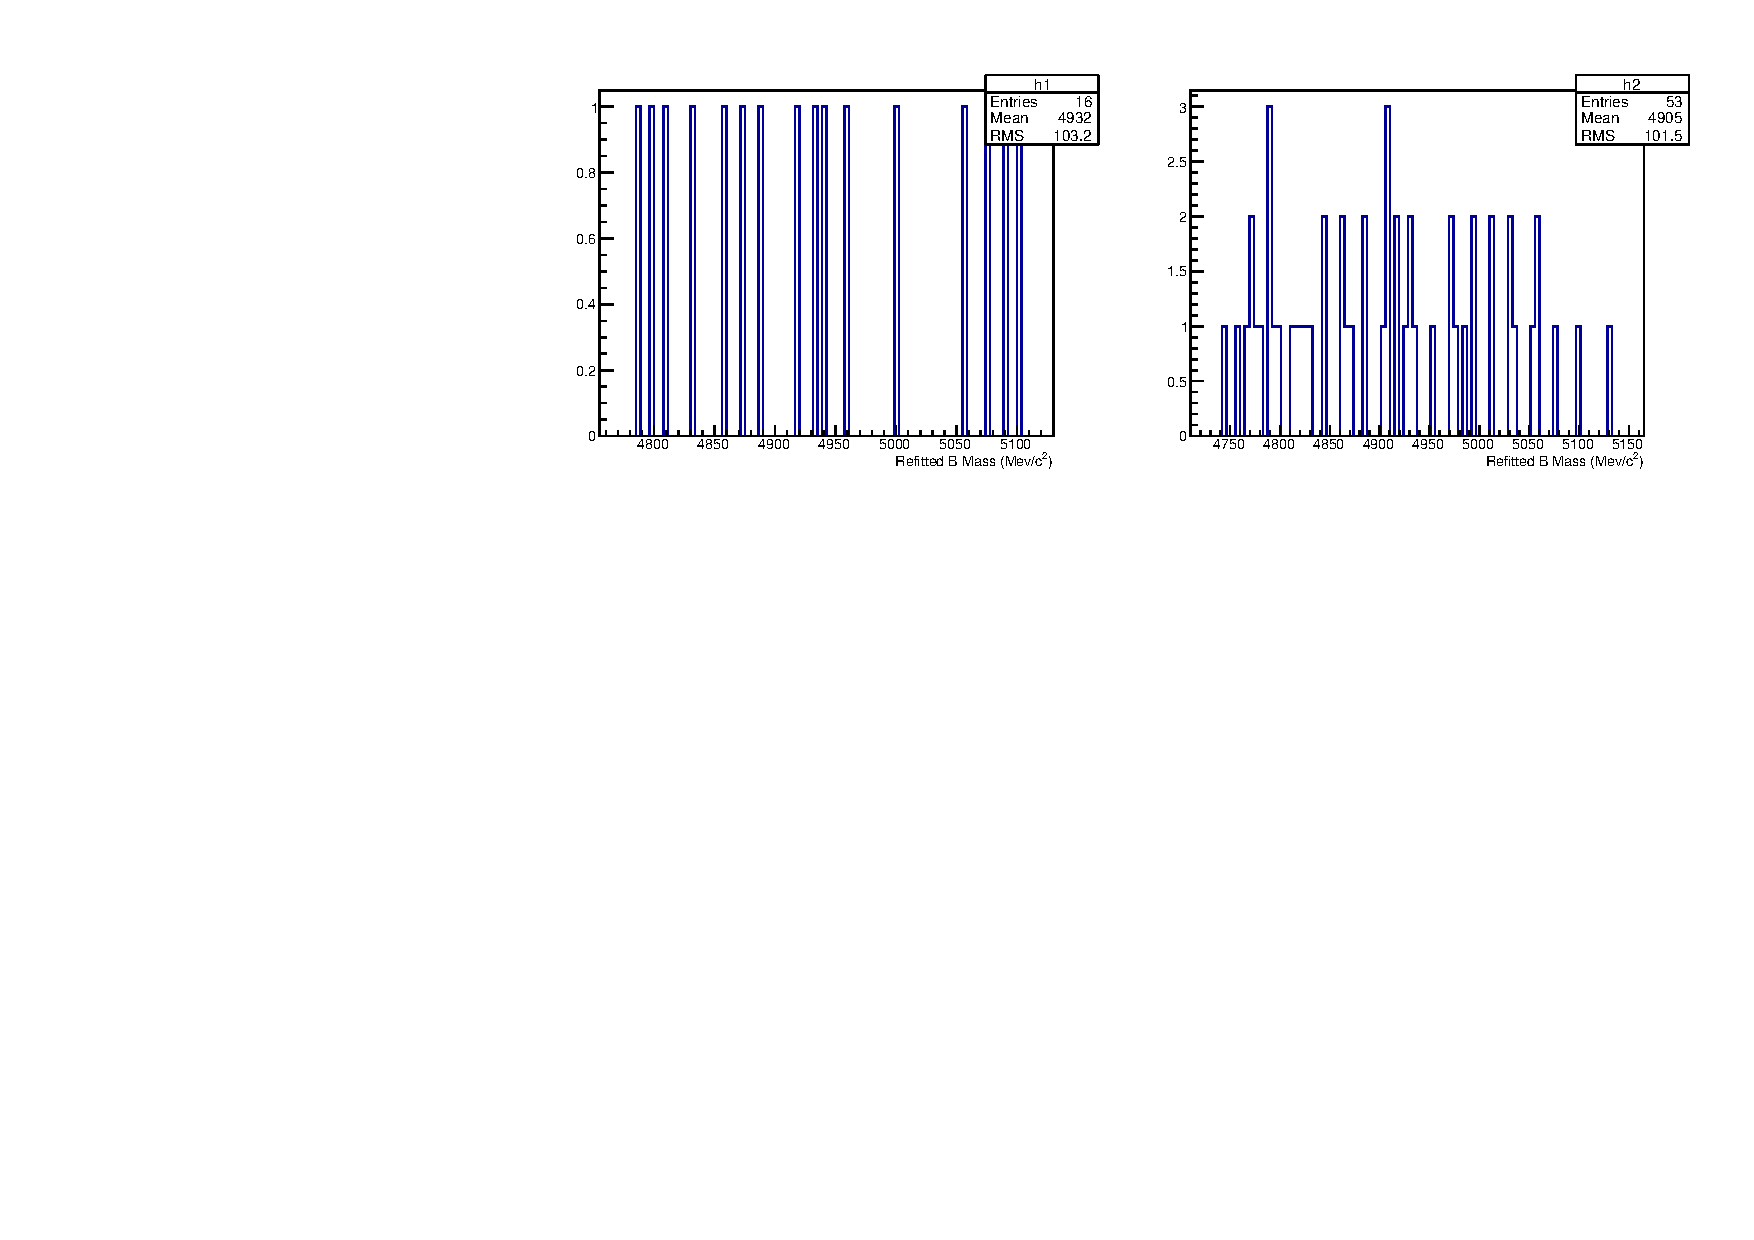
\includegraphics[width=0.7\linewidth]{figures/backgrounds/B2DKstPi0.pdf}
\caption{\decay{\B}{\D\Kstar\piz} MC events remaining after the full selection is applied to 1M generated events}
\label{B2DKstPi0}
\end{figure}

\section{\decay{\B}{\D\KS\kaon}}

The decay \decay{\B}{\D\KS\kaon} has a branching fraction of $5.5 \times 10^{-4}$~\cite{PDG2014}. Figure \ref{B2DKKs} shows the remaining events after applying the full selection to 1M \decay{\B}{\D\KS\kaon} MC events. The estimated contribution in the favoured \decay{\B}{\D(\kaon\pi)\Kstar} mass fit is 0.5\% and 0.4\%, for LL and DD respectively, of the signal in the mass range 4900-5250 MeV. The low mass range for the simultaneous fit is 5230 MeV and so this background is considered negligible.

\begin{figure}[h]
\centering
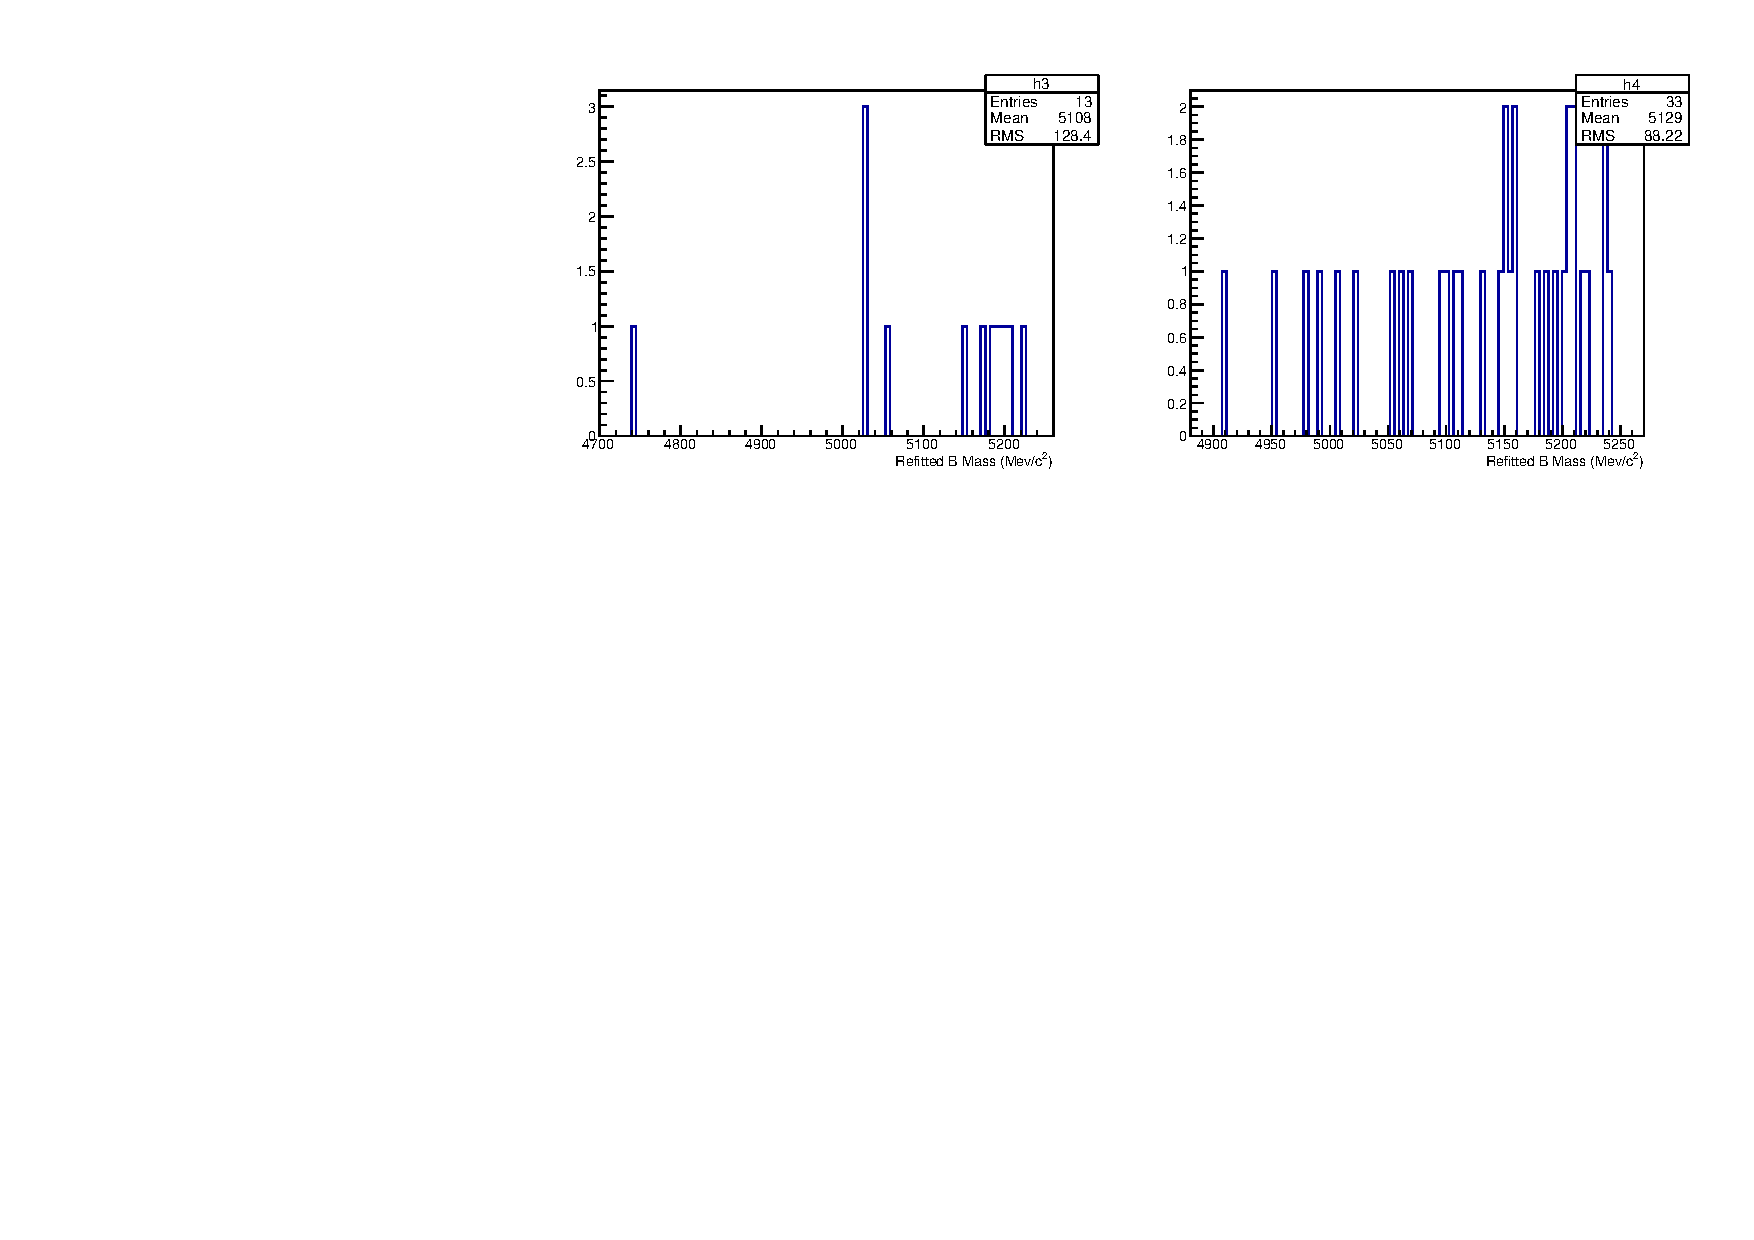
\includegraphics[width=0.7\linewidth]{figures/backgrounds/B2DKKs.pdf}
\caption{\decay{\B}{\D\KS\kaon} MC events remaining after the full selection is applied to 1M generated events}
\label{B2DKKs}
\end{figure}

\section{\decay{\Bs}{\Dz\KS\pi\pi}}

There is no measured branching fraction for \decay{\Bs}{\Dz\KS\pi\pi}. A \decay{\Bs}{\Dz\KS\pi\pi} branching fraction of $5 \times 10^{-4}$ is assumed. The full selection is applied to 0.5M \decay{\Bs}{\Dz\KS\pi\pi} events, Figure \ref{Bs2D0KsPiPi} shows the distribution of the remaining events. The estimated contribution in the favoured \decay{\B}{\D(\kaon\pi)\Kstar} mass fit is 0.4\% and 0.2\% of the signal, for LL and DD respectively, across the mass range 4750-5120 MeV. As the simultaneous fit has a mass range starting from 5230 MeV, this background is not considered for the mass fit.

\begin{figure}[h]
\centering
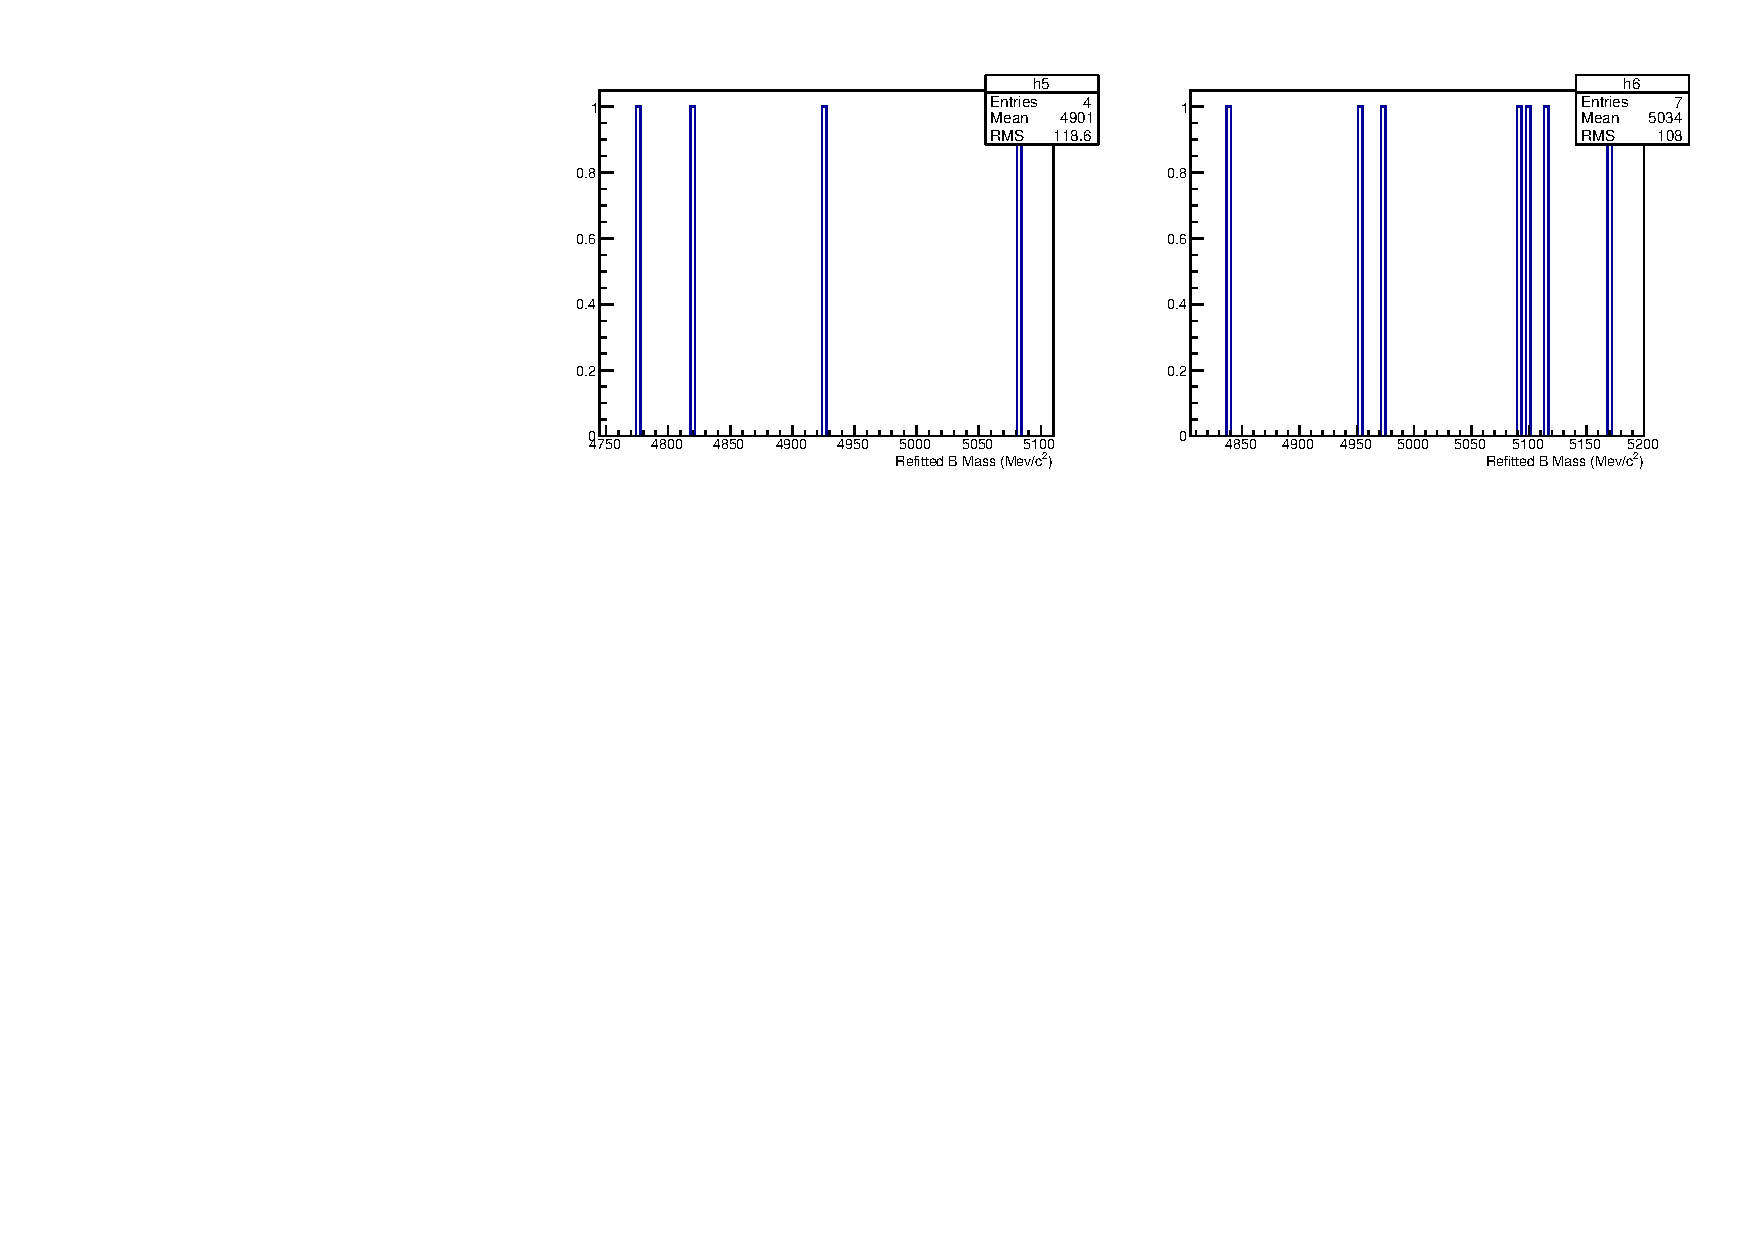
\includegraphics[width=0.7\linewidth]{figures/backgrounds/Bs2D0KsPiPi.pdf}
\caption{\decay{\Bs}{\Dz\KS\pi\pi} MC events remaining after the full selection is applied to 1M generated events}
\label{Bs2D0KsPiPi}
\end{figure}

\clearpage